% Standalone figure: run make in this directory to build PDF and SVG.
\documentclass[11pt,tikz,border=0pt]{standalone}
\usepackage{fontspec}
\IfFontExistsTF{Helvetica Neue Light}{
  \setsansfont{Helvetica Neue Light}[BoldFont={Helvetica Neue Medium}]
  \newfontfamily\vnmedium{Helvetica Neue Medium}
}{
  \setsansfont{TeX Gyre Heros}
  \newcommand{\vnmedium}{\bfseries}
}
\renewcommand{\familydefault}{\sfdefault}
\usepackage{amsmath,amssymb,mathtools}
\usepackage{unicode-math}
\setmathfont{latinmodern-math.otf}
\usetikzlibrary{arrows.meta,calc,positioning}
\definecolor{vnslideink}{HTML}{333333}
\definecolor{vnslidebody}{HTML}{5E5E5E}
\definecolor{vnaccent}{HTML}{FF644E}
\definecolor{vnslidelink}{HTML}{579ACA}
\pagecolor{white}
\tikzset{
  graphvertex/.style={draw=vnslideink,circle,fill=white,line width=0.7pt,
    minimum size=7mm,inner sep=0pt,font=\small\vnmedium},
  graphedge/.style={draw=vnslidebody,line width=0.8pt},
  grapharrow/.style={draw=vnslidebody,line width=0.8pt,-{Latex[length=2.5mm]}},
  graphaccent/.style={draw=vnaccent,line width=1.2pt,-{Latex[length=2.5mm]}},
}

\begin{document}
\color{vnslidebody}
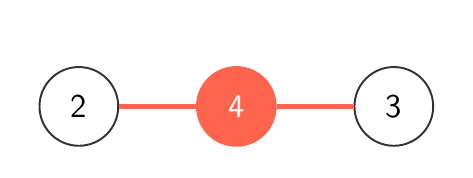
\begin{tikzpicture}[x=1cm,y=1cm,
        degreevertex/.style={graphvertex,minimum size=10mm,font=\large\vnmedium}]
        \node[degreevertex] (u2) at (0,0) {2};
        \node[degreevertex,fill=vnaccent,draw=vnaccent,text=white] (u4) at (2,0) {4};
        \node[degreevertex] (u3) at (4,0) {3};
        \draw[draw=vnaccent,line width=1.6pt] (u2)--(u4);
        \draw[draw=vnaccent,line width=1.6pt] (u4)--(u3);
        \path[use as bounding box] (-0.65,-0.55) rectangle (4.65,1.0);
      \end{tikzpicture}
\end{document}
